% TODO : Fix x,y-axis labels 
\begin{figure}[h]
    \centering
    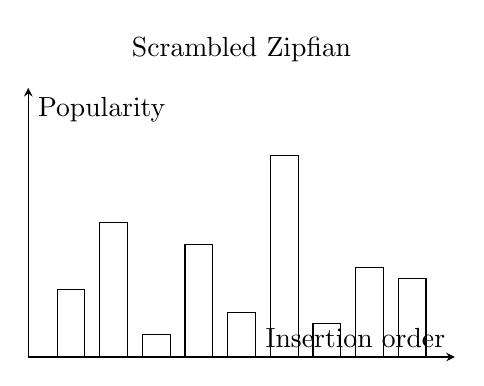
\begin{tikzpicture}
        \begin{axis}[
            width=7cm,
            height=5cm,
            title={Scrambled Zipfian},
            xlabel style={at={(axis description cs:0.5,-0.1)},anchor=north},
            ylabel style={at={(axis description cs:-0.1,.5)},rotate=90,anchor=south},
            xlabel={Insertion order},
            ylabel={Popularity},
            xtick=\empty,
            ytick=\empty,
            axis lines=middle,
            ymin=0, ymax=1.2,
            xmin=0, xmax=10
        ]
        \addplot[ybar,fill=white,draw=black] coordinates {(1,0.3) (2,0.6) (3,0.1) (4,0.5) (5,0.2) (6,0.9) (7,0.15) (8,0.4) (9,0.35)};
        \end{axis}
    \end{tikzpicture}
    \hspace{1cm}
    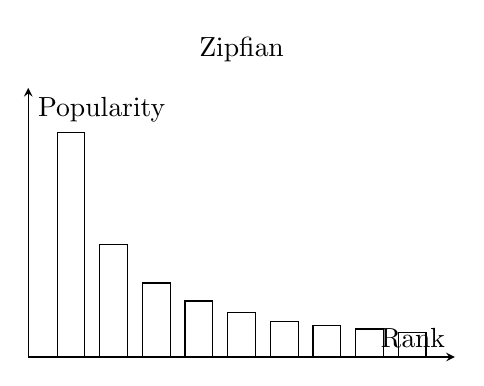
\begin{tikzpicture}
        \begin{axis}[
            width=7cm,
            height=5cm,
            title={Zipfian},
            xlabel style={at={(axis description cs:0.5,-0.1)},anchor=north},
            ylabel style={at={(axis description cs:-0.1,.5)},rotate=90,anchor=south},
            xlabel={Rank},
            ylabel={Popularity},
            xtick=\empty,
            ytick=\empty,
            axis lines=middle,
            ymin=0, ymax=1.2,
            xmin=0, xmax=10
        ]
        \addplot[ybar,fill=white,draw=black] coordinates {(1,1) (2,0.5) (3,0.33) (4,0.25) (5,0.2) (6,0.16) (7,0.14) (8,0.125) (9,0.11)};
        \end{axis}
    \end{tikzpicture}
    \caption{Comparison of Jim Gray's version (right) and the one employed by YCSB (left).}
    \label{fig:zipfian_comparison_ycsb}
\end{figure}